\documentclass[11pt]{article}
\usepackage{lineno}
\usepackage{graphicx}
\usepackage{bm}

\begin{document}

\begin{titlepage}

\newcommand{\HRule}{\rule{\linewidth}{0.5mm}} 

\center % Center everything on the page
 
%----------------------------------------------------------------------------------------
%	HEADING SECTIONS
%----------------------------------------------------------------------------------------

\textsc{\LARGE Texas A$\&$M University}\\[1.5cm] 
\textsc{\Large Summer Research Paper 1}\\[0.5cm] % 

%----------------------------------------------------------------------------------------
%	TITLE SECTION
%----------------------------------------------------------------------------------------

\HRule \\[0.4cm]
{ \huge \bfseries Exploring the Euclidean Algorithm}\\[0.4cm] 
\HRule \\[1.5cm]
 
%----------------------------------------------------------------------------------------
%	AUTHOR SECTION
%----------------------------------------------------------------------------------------

\begin{minipage}{0.4\textwidth}
\begin{flushleft} \large
\emph{Authors:}\\
Stephen \textsc{Capps}\\
Sarah \textsc{Sahibzada}\\
Taylor \textsc{Wilson}
\end{flushleft}
\end{minipage}
~
\begin{minipage}{0.4\textwidth}
\begin{flushright} \large
\emph{Supervisor:} \\
Dr. Sarah \textsc{Pollock} 
\end{flushright}
\end{minipage}\\[4cm]

%----------------------------------------------------------------------------------------
%	DATE SECTION
%----------------------------------------------------------------------------------------

{\large \today}\\[3cm] 

%----------------------------------------------------------------------------------------
%	LOGO SECTION
%----------------------------------------------------------------------------------------

%\includegraphics{Logo}\\[1cm] 
 
%----------------------------------------------------------------------------------------

\vfill 

\end{titlepage}

\tableofcontents
\newpage
\newpage

\section{Introduction}
$ $ \indent The Euclidean Algorithm is familiar to most, and is widely used in many fields, such as cryptography and number theory. Aging over two millennia, it has raised many questions over its lifetime. This paper will specifically investigate the number of iterations it takes to complete the Euclidean Algorithm. 

For example, the number of iterations it take to complete gcd$(42,36)$ is $2$, as shown below.
		$$\mathrm{gcd}(42,36) = 6:$$

	\begin{equation}
		42 = 1 * 36 + 6
	\end{equation}
	\begin{equation}
		36 = 6 * 6 + 0
	\end{equation}
Some other examples are as follows:

\begin{center}
\begin{tabular}{c|c}

$\mathrm{gcd}(\mathrm{p},\mathrm{q}) = \mathrm{d}$ & Iterations
\\
\hline
$\mathrm{gcd}(689,456) = 1$ & $6$\\

$\mathrm{gcd}(78,45) = 3$ & $5$\\

$\mathrm{gcd}(8394,238) = 2$ & $7$\\


\end{tabular}
\end{center}




This leads us to an investigation into what numbers yield the longest iterations, and the distribution of these iterations.


\section{Theoretical Analysis}$ $


\section{Computational Approaches}$ $
While the nature of this investigation makes the exploration of sets of numbers with n digits a logical approach to understanding the Euclidean algorithm, the computational run-time of any algorithm is measured in terms of the size of input in terms of a unit fundamental to computing called a bit, which represents a power of two. This allows for the correction of confounding variables in measuring the running time of implementations of algorithms: the language and platform used are just two of many factors which might cause variation in the running time of an algorithm. The running time of an algorithm is thus measured in terms of the number of bit-wise operations executed throughout the duration of the algorithm and, consequently, asymptotic functions are typically used to approximate the number of necessary bitwise operations taken for an input of size n bits. We define the below notation, typically termed Big-O notation, as an asymptotic upper bound on the run time of an algorithm implementation in terms of the input size:
\\ \indent Definition: f = O(g(n)) iff there exists a positive constant k as well as a positive integer n0 for which 0 ≤ f(n) ≤ k(g(n)), for all n ≥ n0. Informally, this means that g(n) provides an asymptotic upper bound for f.\\
\indent Consequently, the term “running time” is somewhat of a misnomer: while it is certain that the time taken for an algorithm to run will be dependent on the input size, the term running time will henceforth be taken to mean the number of bitwise operations taken for an algorithm to execute. 
\\ \indent The computational complexity of all algorithms surveyed will be phrased in the above notation and, by extension, will fundamentally be expressed in terms of the computational expense of bitwise operations. As a result, running time data generated from any future implementations of these algorithms may be analyzed in terms of a fundamental constant. For clarity, basic assumption the bit complexity of the basic operations in the ring of integers, as well as a function determining the number of bits in a number, will be defined.\\
\\
\indent The number of bits in the binary representation of a number is related to the base-2 logarithm of that number.\\


Definition: The binary representation of a number n will have m bits where m is given by:
	$$m = 1 + \mathrm{floor}(\mathrm{log}2n)\quad \mathrm{iff}\quad n \neq 0$$
	$$m = 1\quad \mathrm{iff}\quad n = 0$$
\indent The value of m may be approximated by log2n. The standard accepted bit complexities for the ring operations for integers, addition and subtraction, as well as their inverses, multiplication and division, are given below:
\begin{center}
\begin{tabular}{c|c|c}

	Operation & Bit Complexity & O(n)\\
	\hline
	a + b &  loga + logb & O(logn)\\
	a - b &  loga - logb & O(logn)\\
	a * b &  (loga)(logb) & O($\mu$(logn))\\
	\\
	a = Qb + R & (logQ,logb) & O($\mu$(logQ,logn))
	
\end{tabular}
\end{center}
\begin{displaymath} where \quad \mu(m,n) = \left\{
	\begin{array}{c c}
	m(logn)(log(logn) & m > n\\
	n(logm)(log(logm) & m < n\\
	\end{array}
	\right. 
\end{displaymath}
\\
\begin{center}
System Background and Terminology
Implementation Details:
\end{center}
 

\indent
All algorithm implementations in this section were performed in Java, a high-level, platform-independent object-oriented language, in order to take advantage of the BigInteger library, a library which allows immutable integers of arbitrary precision and contains all standard arithmetic operations allowed for integers in this language as well as tests for primality. In order to automate the generation of data sets from the algorithms implemented, several scripts in Bash, a cross-platform scripting language, were also developed. The implementations were run on a Linux-based server hosed through the Department of Computer Science at Texas A$\&$M University; the average running time of elementary operations was timed on this server and is given below:

The term “iterations” will refer to a consecutive sequence of operations to generate the next set of values used by the algorithm; in any iterative version, this will refer to the three fundamental steps that occur in each loop, and in any recursive version, this will refer to one recursive call.
Algorithms: Overview
Several variants of the Euclidean algorithm were studied for purposes of this investigation. In particular, three iterative versions, two recursive versions, and two binary versions were implemented. The first, the so-called classical Euclidean algorithm, performs successive subtractions on the input pairs of numbers in order to compute their greatest common divisor.  An improvement to the subtractive algorithm due to Lame will reduce the number of subtractive steps, and finally, the modulo operation will consolidate this process in order to return the remainder. Two recursive versions: a recursive version of the modular algorithm, as well as an improvement upon this version, were implemented as well. Finally, binary versions of the algorithm were implemented.
Algorithms: Detail
Process
The algorithms were all run on a data set containing the first 1000 Fibonacci numbers, and their running times measuered in terms of the number of iterations taken as well as the total running time of the algorithm. A similar set of data was collected on each algorithm on a set of randomly-generated 100-digit numbers. 


\section{Results}$ $	\indent The results were quiet surprising, as most distributions were almost perfectly Gaussian. The following figures are different distributions of different iterations of various gcd combinations.\\
	
	\begin{figure}
		
		\center 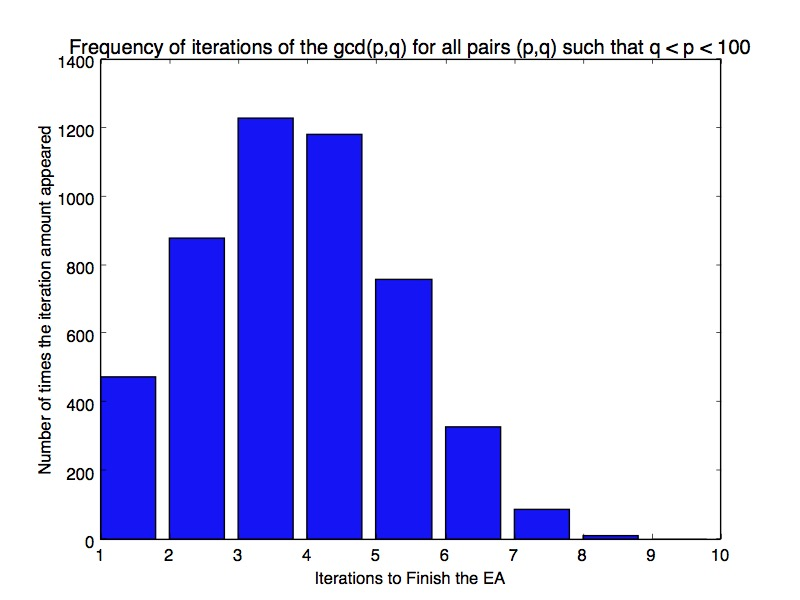
\includegraphics[scale=.4]{2digit_iterationfreq.jpg}
		\center \tiny(Figure 1)\\
		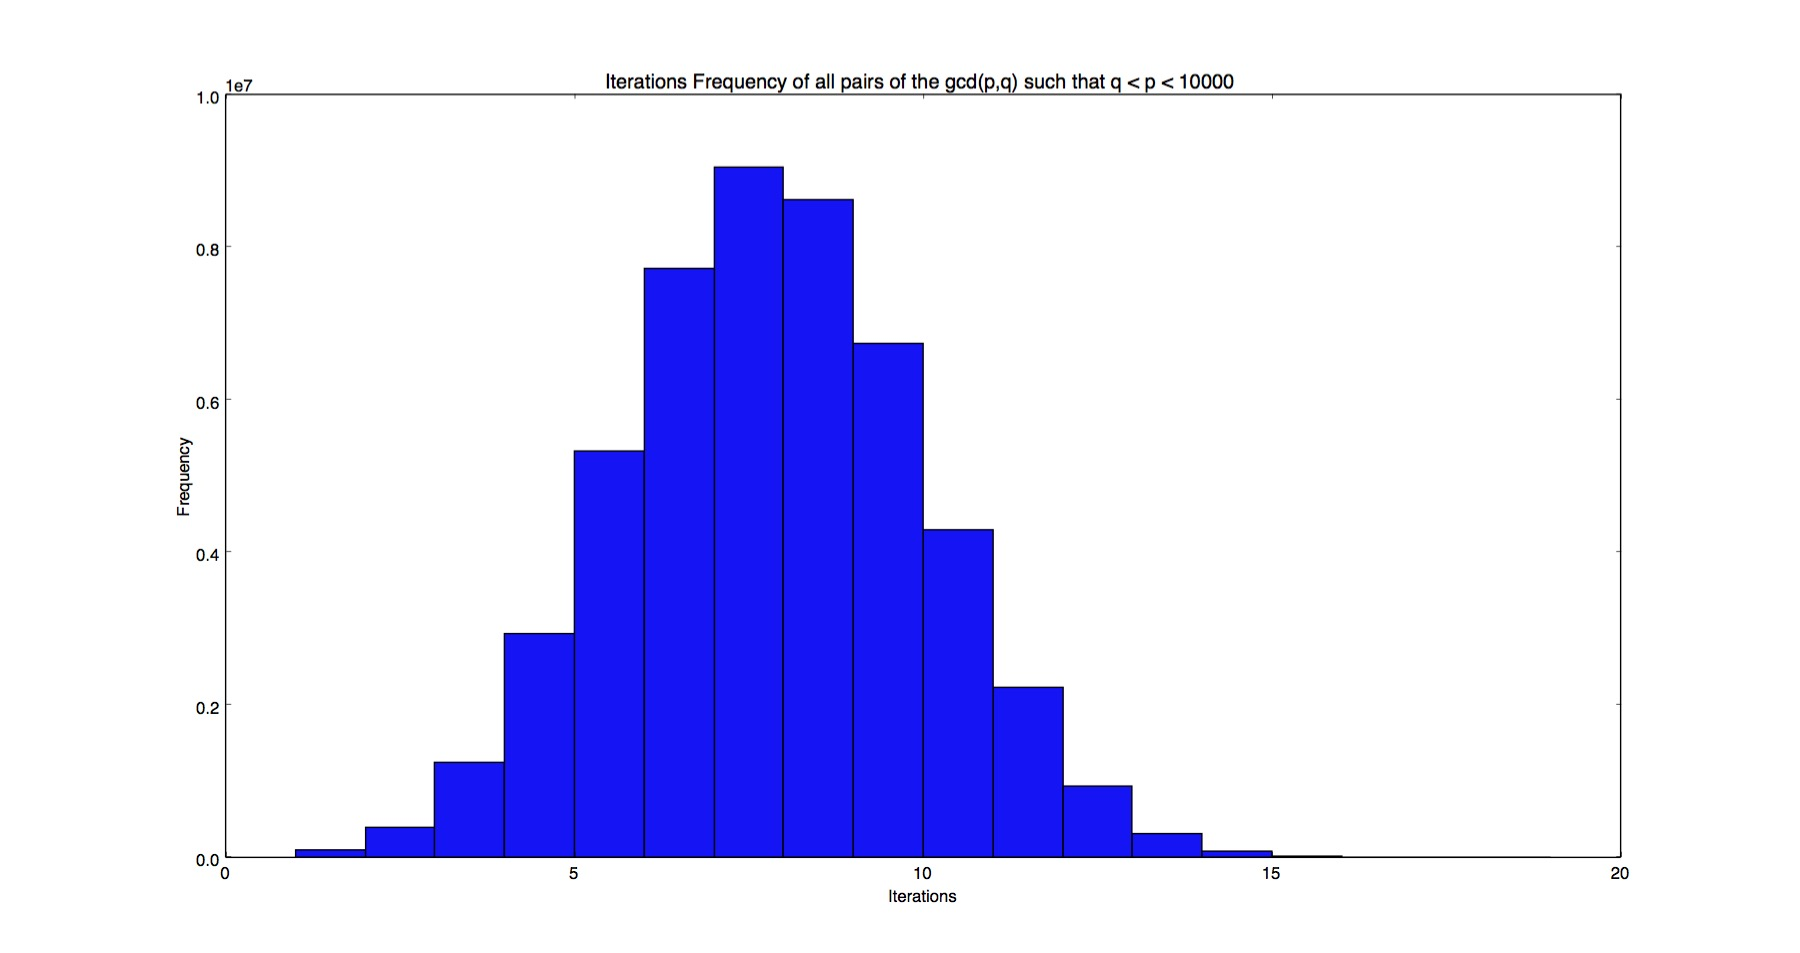
\includegraphics[scale=.4]{4digit_iteration_freq.jpg}
		\center \tiny(Figure 2)
	\end{figure}
	
	\begin{figure}
		\center
		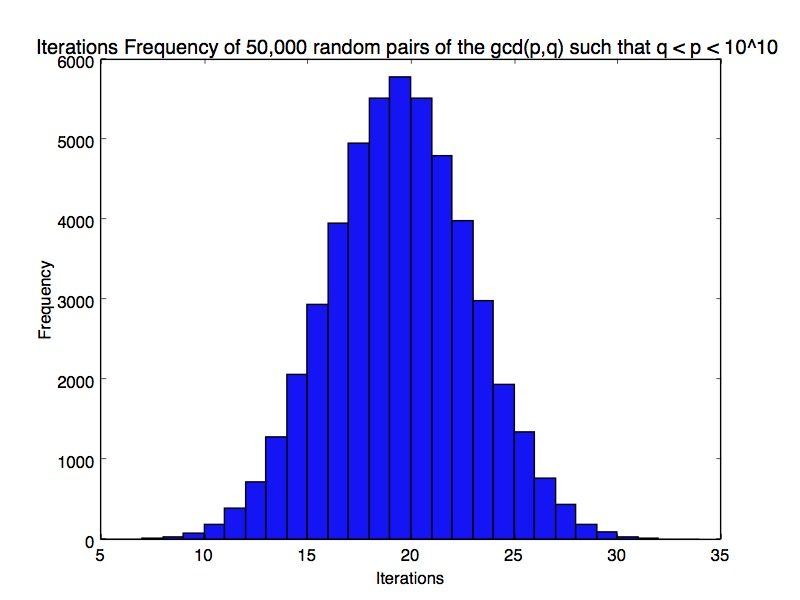
\includegraphics[scale=.4]{10_digit_numbers.jpg}
		\center \tiny(Figure 3)\\
			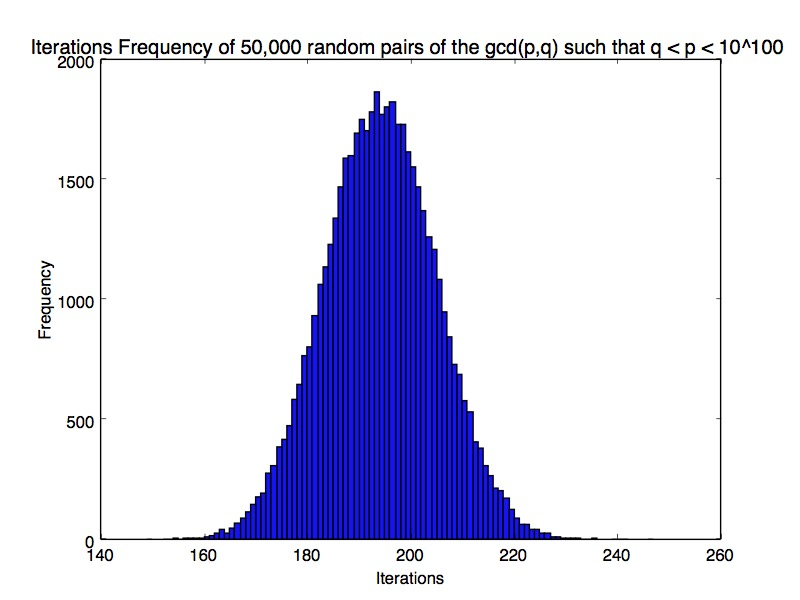
\includegraphics[scale=.4]{100_digit_numbers_freq.jpg}
		\center \tiny(Figure 4)
		
	\end{figure}
	
	
	
	\begin{figure}
		\centering

		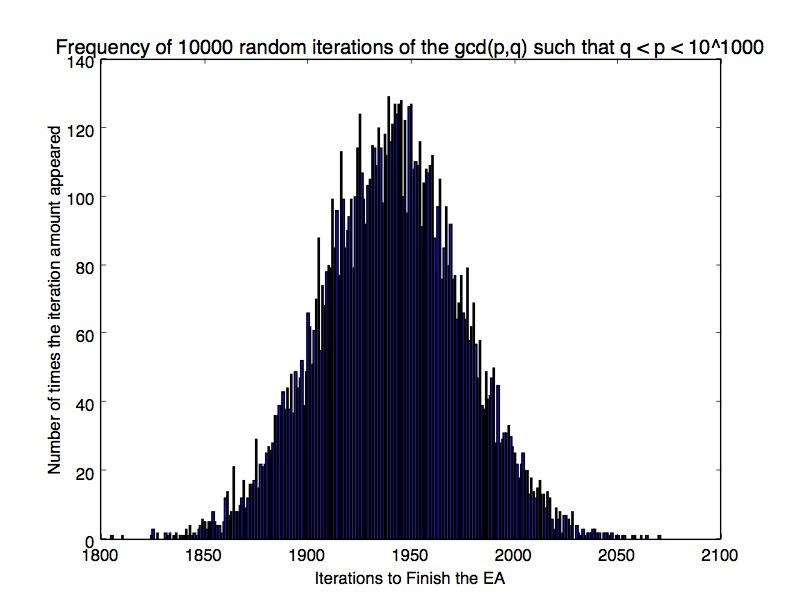
\includegraphics[scale=.4]{1000_digit_numbers.jpg}
		\center \tiny(Figure 5)
		
	\end{figure}
	\newpage
	As the number of digits we consider increases, the distribution	 becomes continuously more Gaussian. However, after a point our computational resources restrict us from checking all pairs p,q with some large upper bound. Thus, we restrict ourselves by picking a set amount of pairs and calculating their distribution. You can see this progression as the figures continue.\\
	
	There are a few minor observations to be made:\\
	
	 First, in (Figure 1), it must be noted that the lack of normality here is due to the small sample size. The size of this data set was no more than $4950$, and spanned across $9$ bins. As the number of bins needed increases, the more normal the graph becomes. 
	
	 Second, in (Figure $5$), the inconsistencies in the normal distribution can be attributed to a too small a sample size. If given the computing power and time, one could compute all pairs less than $10^{1000}$. Note the increasing mean iterations as we climb the upper bound.
\section{Discussion}$ $
\indent As it is obvious, the distribution of these gcd lengths is almost perfectly Gaussian. The approach we used seemed to work awfully well, as computers handle modular operations and subtraction very well. The main constraints we had were as we went past $5$ digit numbers. Calculating all pairs becomes exponentially difficult as the digits you allow increases. 



\section{Individual Contributions}$ $





\end{document}